\documentclass[letterpaper,12pt,]{article}

\usepackage{titling}

\setlength{\droptitle}{5in}   % This is your set screw

\usepackage[%
    left=1in,%
    right=1in,%
    top=1in,%
    bottom=1.0in,%
    paperheight=11in,%
    paperwidth=8.5in%
]{geometry}%
\usepackage{comment}

\usepackage{listings}
\usepackage{graphicx}
\usepackage{amsmath}
\usepackage[section]{placeins}
\usepackage[font=small,skip=0pt]{caption}
\usepackage{subcaption}
\usepackage{hyperref}
\usepackage{booktabs}
\usepackage{pdfpages}


\lstdefinestyle{mystyle}{
    %backgroundcolor=\color{backcolour},
    %commentstyle=\color{codegreen},
    %keywordstyle=\color{magenta},
    %numberstyle=\tiny\color{codegray},
    %stringstyle=\color{codepurple},
    basicstyle=\footnotesize,
    breakatwhitespace=false,
    breaklines=true,
    captionpos=b,
    keepspaces=true,
    numbers=left,
    numberstyle=\footnotesize,
    stepnumber=1,
    numbersep=5pt,
    showspaces=false,
    showstringspaces=false,
    showtabs=false,
    tabsize=2,
    frame=single
}
\lstset{frame=single}

\pagestyle{empty} % Remove page numbering
\linespread{1.5} % Line Spacing

\begin{document}

\begin{titlepage}

\newcommand{\HRule}{\rule{\linewidth}{0.5mm}} % Defines a new command for the horizontal lines, change thickness here

\center % Center everything on the page
 
%----------------------------------------------------------------------------------------
%	HEADING SECTIONS
%----------------------------------------------------------------------------------------


\textsc{\LARGE McGill University}\\[3.5cm]
\textsc{\Large Computational Aerodynamics}\\[0.5cm] 
\textsc{\large MECH 539}\\[2.5cm]

%----------------------------------------------------------------------------------------
%	TITLE SECTION
%----------------------------------------------------------------------------------------

{ \huge \bfseries Project 2}\\[1.5cm] % Title of your document

\HRule \\[0.4cm]
%----------------------------------------------------------------------------------------
%	AUTHOR SECTION
%----------------------------------------------------------------------------------------

\begin{minipage}{0.4\textwidth}
\begin{flushleft} \large
\emph{Name:}\\
Doug \textsc{Shi-Dong} % Your name
\end{flushleft}
\end{minipage}
~
\begin{minipage}{0.4\textwidth}
\begin{flushright} \large
\emph{Student ID:} \\
260466662\\
\end{flushright}
\end{minipage}\\[4cm]

\vfill{}
{\large February 18, 2016}\\[2cm]

\end{titlepage}


\section*{Question 1: Grid Study}

\begin{figure}[!h]
    \centering
    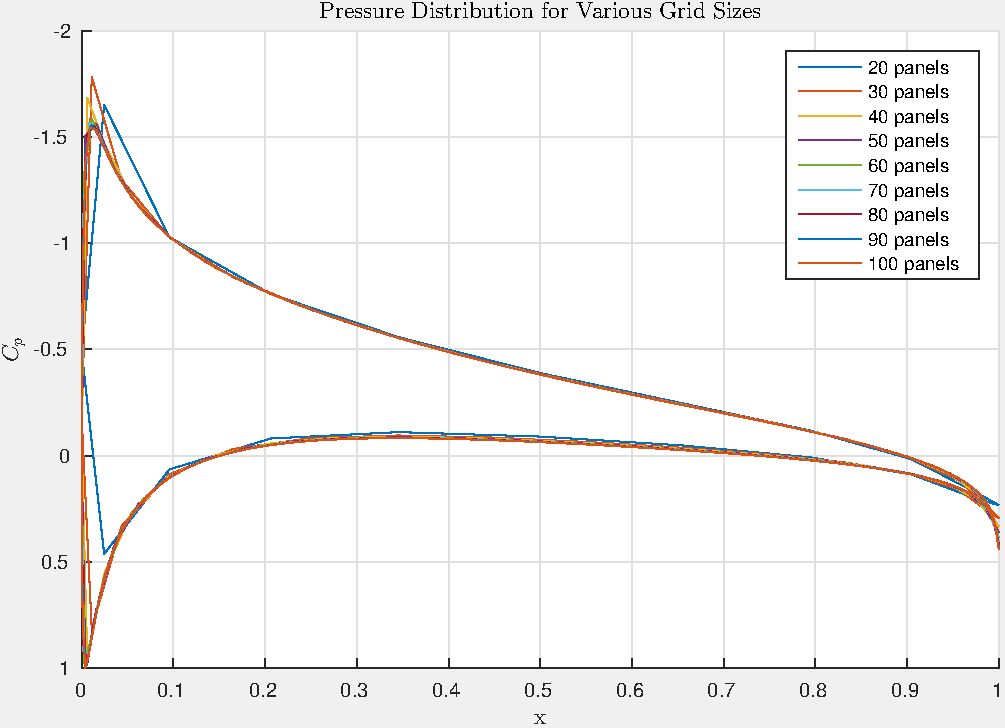
\includegraphics[width = 0.95\textwidth]{./figures/q1pressure.pdf}
    \caption{Pressure Distribution NACA0012, $Re = 1\textsc{e}06$, $\alpha = 4^{\circ}$}
    \label{fig:q1p}
\end{figure}

The pressure distribution for various number of panels is shown in Figure \ref{fig:q1p}.
As the number of panels increase, the pressure distribution converges to a smoother shape.
It is possible to visually differentiate the pressure distribution of 20, 30 and 40 panels from the other results.

The lift and drag coefficients are compiled in Table \ref{tab1}.
Their convergence are graphically shown in Figure \ref{fig:q1l} and \ref{fig:q1d}.
As the number of panels increases, the lift and drag coefficients also converge.
For lower numbers of panels, the drag coefficient is higher than its converged value and the lift coefficient is lower than its converged value.
Since less panels entails a bigger grid spacing, the truncation error is higher for coarser grids.
Numerical dissipation has stronger effects for coarse grids, resulting in weaker performances of the airfoil.

From Figure \ref{fig:q1l} and \ref{fig:q1d}, 30-40 panels seem to be sufficient to get a reasonably accurate lift coefficient, while 50 panels are required to get an accurate drag coefficient.

\begin{table}[!h]
\centering
\begin{tabular}{ccc} \toprule
    {Number of Panels} & {$C_L$} & {$C_D$} \\ \midrule
    {20} & 0.4488  & 0.0093\\
    {30} & 0.4673  & 0.0095\\
    {40} & 0.4724  & 0.0095\\
    {50} & 0.4746  & 0.0084\\
    {60} & 0.4759  & 0.0083\\
    {70} & 0.4768  & 0.0083\\
    {80} & 0.4774  & 0.0082\\
    {90} & 0.4778  & 0.0083\\
    {100} & 0.4782  & 0.0082 \\
\bottomrule
\end{tabular}
\caption{Lift and Drag Coefficients for NACA0012, $Re = 1.00\textsc{e}06$, $\alpha = 4^{\circ}$}
\label{tab1}
\end{table}

\begin{figure}[!h]
    \centering
    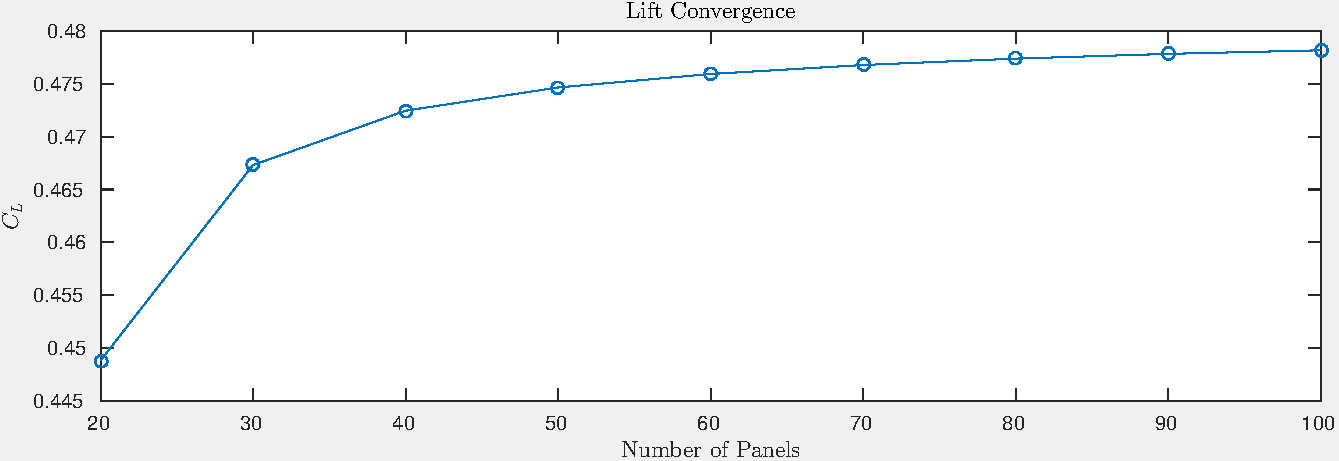
\includegraphics[width = 0.95\textwidth]{./figures/q1lift.pdf}
    \caption{Lift Grid Study}
    \label{fig:q1l}
\end{figure}

\begin{figure}[!h]
    \centering
    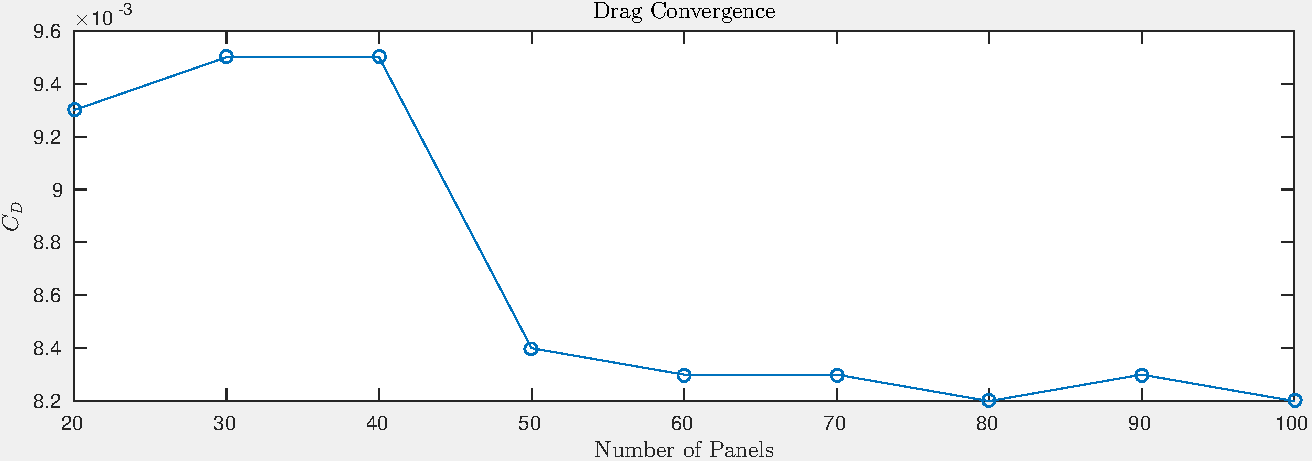
\includegraphics[width = 0.95\textwidth]{./figures/q1drag.pdf}
    \caption{Drag Grid Study}
    \label{fig:q1d}
\end{figure}

\section*{Question 2: Pressure Validation}

\begin{figure}[!h]
    \centering
    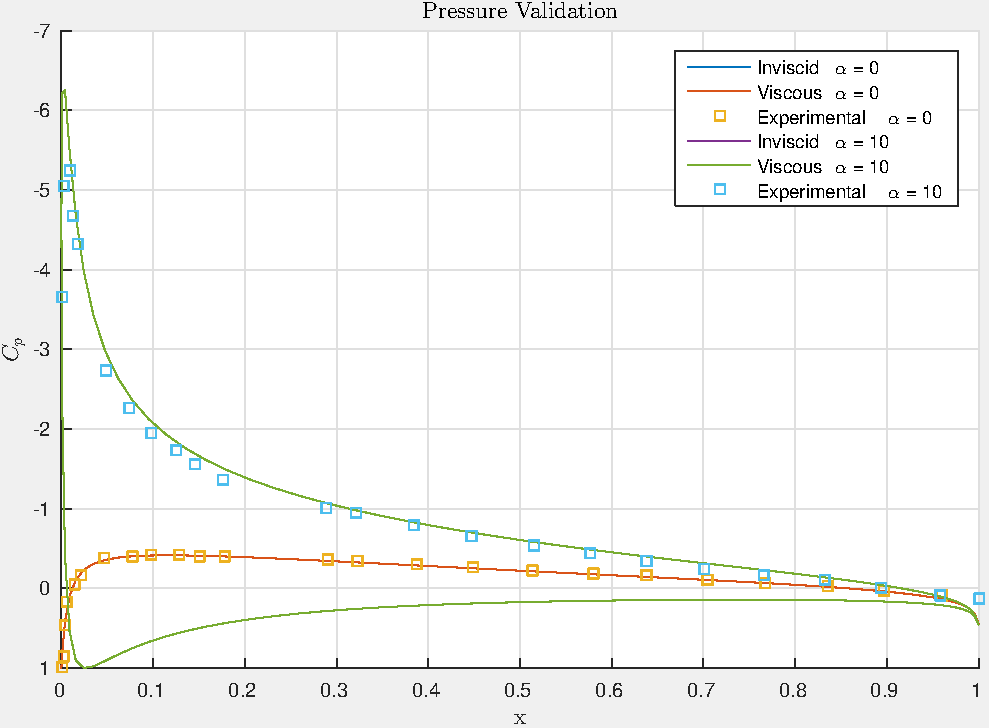
\includegraphics[width = 0.95\textwidth]{./figures/q2pressure.pdf}
    \caption{Drag Grid Study}
    \label{fig:q2}
\end{figure}

Figure \ref{fig:q2} shows numerical and experimental solutions of the NACA0012 at an angle of attack $\alpha = 0^\circ$ and $\alpha = 10^\circ$ with $Re = 2.88\textsc{e}06$.
The pressure distribution from the inviscid and viscous runs are exactly the same. Since the solver does not iterate between the solutions of the flow field and the boundary layer, the same flow field is solved in the first place.

For $\alpha = 0^\circ$ the pressure distribution is the same on lower and upper surface as expected due to symmetry. For $\alpha = 10^\circ$ the pressure distribution shows a negative pressure on the upper surface and a positive pressure on the lower surface, creating lift.

The potential flow solver is surprisingly accurate when it is compared with experimental data from Gregory \& O'Reilly.
This is because the assumption of inviscid, incompressible and irrotational flow are valid for this flow regime.
It can be noticed that those assumptions start to be less adequate for a higher angle of attack.

\section*{Question 3: Angle of Attack Study}

\subsection*{(a) Pressure Distribution}
\begin{figure}[!h]
    \centering
    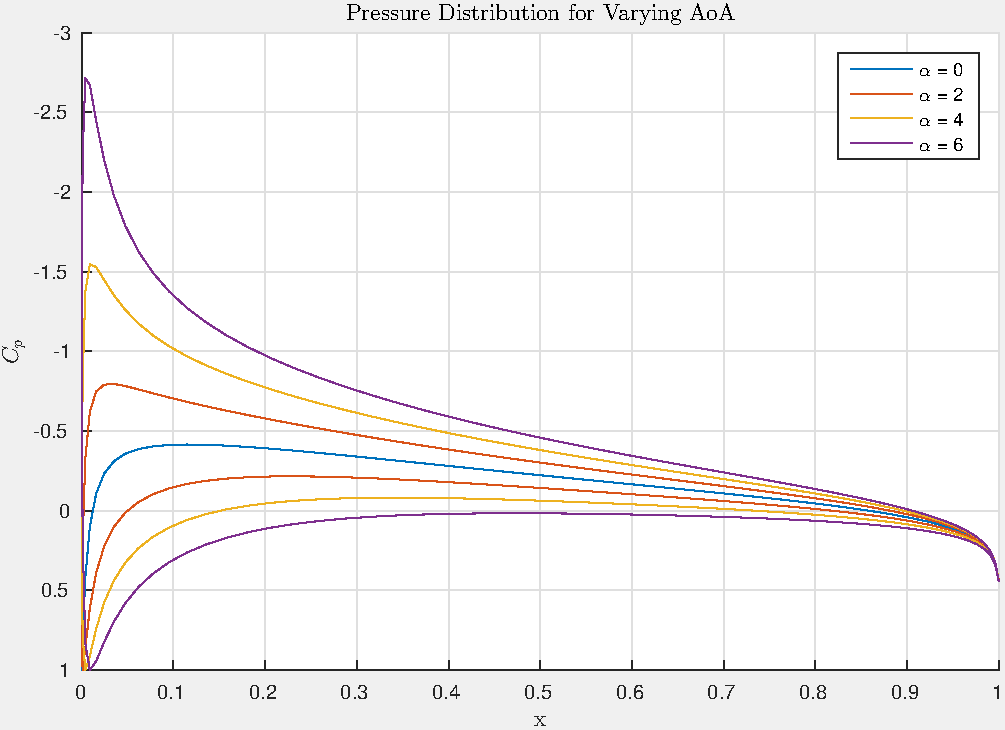
\includegraphics[width = 0.95\textwidth]{./figures/q3pressure.pdf}
    \caption{Pressure Distribution of NACA0012}
    \label{fig:q3p}
\end{figure}

Figure \ref{fig:q3p} shows the pressure distribution of the NACA0012 for varying AoA's.
As the AoA increases so does the pressure difference between the lower and upper surface.

An increasing AoA exposes the lower surface more directly to the incoming flow, resulting in a lower velocity and higher pressure. Meanwhile, the upper surface requires a faster turn at the leading edge, resulting in a lower pressure.

\subsection*{(b) Drag Polar}
\begin{figure}[!h]
    \centering
    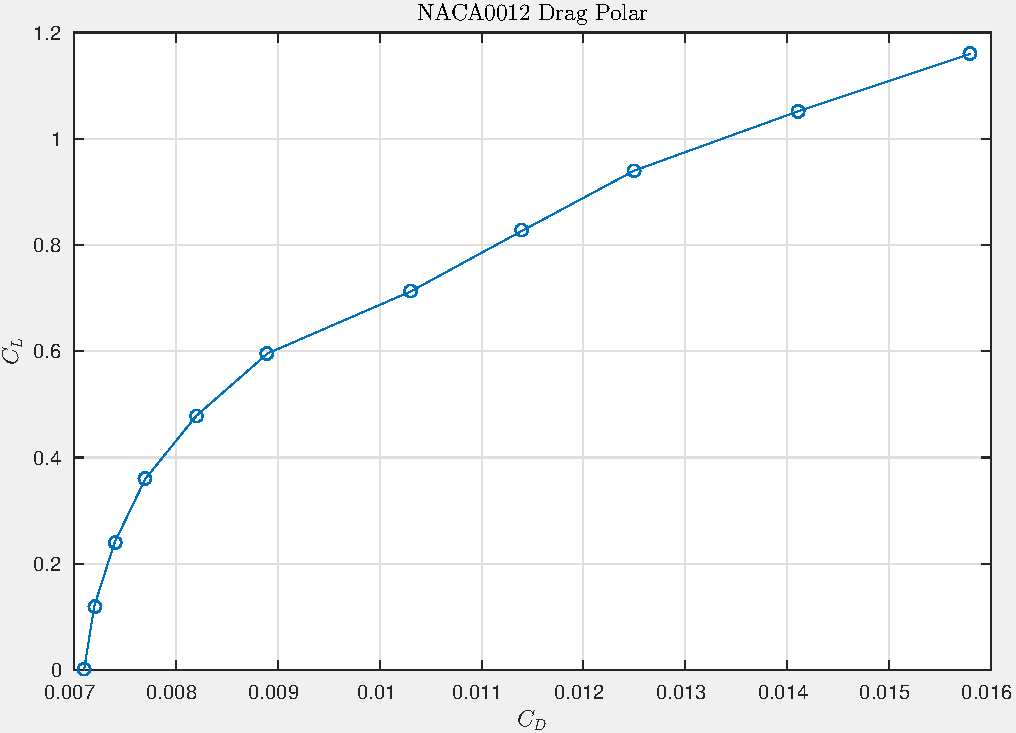
\includegraphics[width = 0.95\textwidth]{./figures/q3dp.pdf}
    \caption{Drag Polar of NACA0012}
    \label{fig:q3dp}
\end{figure}

Figure \ref{fig:q3dp} shows the drag polar of the NACA0012 for $\alpha = \left[0^\circ,10^\circ\right]$.

\subsection*{(c) Effect on Drag}

As the AoA increases, the drag coefficient increases as well.
The lower AoA shows a quadratic increase in drag as the lift increases.
However, the drag polar plot becomes linear starting around $\alpha = 4^\circ$.

The only source of drag present in this solver is skin friction drag, which should be linearly proportional to the coefficient of lift.

\section*{Question 4}

\subsection*{(a) Drag Polar}
\begin{figure}[!h]
    \centering
    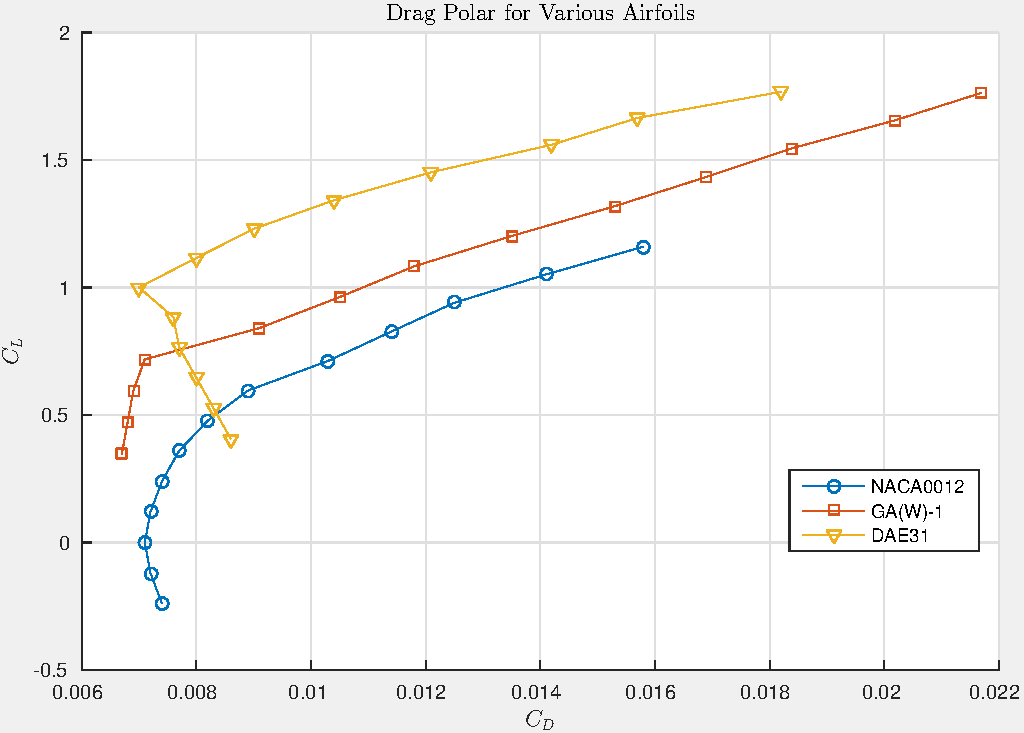
\includegraphics[width = 0.95\textwidth]{./figures/q4dp.pdf}
    \caption{Drag Polar of Various Airfoils}
    \label{fig:q4a}
\end{figure}

The drag polar for the NACA0012, GA(W)-1 and DAE31 are shows in Figure \ref{fig:q4a}.

The NACA0012 has negative lift for negative AoA's since it is a symmetric airfoil. Increasing the AoA in the positive direction leads to higher lift and drag coefficients.

The GA(W)-1 has positive lift for negative AoA's.
As the AoA increases, both the lift and drag coefficients increase.
The slope of the drag polar shows that it is favorable to increase the AoA until $1^\circ$ since a lot of lift is gained for very little drag.

The DAE31 has an even better performance than the previous two airfoils.
Negative AoA's have positive lift coefficients.
Between $-2^\circ$ and $3^\circ$, the drag coefficient decreases while the lift coefficient increases.

An interesting feature to note is that after the initial lift-to-drag improvement, all three drag polars have the same slope, showing the linear proportionality of skin friction drag to lift. Figure \ref{fig:q4a} shows the obvious superiority of the DAE31, followed by the GA(W)-1, followed by the NACA0012 once the initial lift-to-drag improvement is reached.

\subsection*{(b) Equivalent Lift}
Table \ref{tab2} compiles the AoA required to achieve $C_L = 1.000$ and its corresponding drag coefficient $C_D$.
It supports the superiority of the DAE31, GA(W)-1  NACA0012 airfoils in this order in a flow with $Re = 1.00\textsc{e}06$ and a required $C_L = 1.000$.

\begin{table}[!h]
\centering
\begin{tabular}{ccc} \toprule
    {Airfoil} & {AoA} & {$C_D$} \\ \midrule
    {NACA0012} & 8.537  & 0.0133\\
    {GA(W)-1} & 3.310  & 0.0109\\
    {DAE31} & 2.998  & 0.0070\\
\bottomrule
\end{tabular}
\caption{Drag Coeffcients for an Equivalent Lift $C_L = 1.000$}
\label{tab2}
\end{table}

\subsection*{(c) Pressure Distribution}

Figure \ref{fig:q4c} shows the pressure distribution for the same three airfoils at an AoA $\alpha = 4^\circ$.
The NACA0012's lower surface is almost entirely a region of favorable pressure gradient until the trailing edge (TE). However, the upper surface is almost entirely a region of adverse pressure gradient except the leading edge (LE).

The GA(W)-1 has a change in pressure gradient on both its upper and lower surface at about 55\% of the chord.
Before this turning point, the pressure gradient was slightly adverse for its upper surface and slightly favorable on its lower surface.
Past the 55\% chord length, the adverse pressure gradient becomes stronger on the upper surface and an adverse pressure gradient develops on its lower surface.
Those phenomena can be explained by the start of the cusp changing the curvature of the airfoil in this area.

The DAE31's lower surface has very little change in pressure along its chord. The upper surface shows a small adverse pressure gradient until about 55\% of the chord. The pressure gradient then increases higher than the one of the GA(W)-1.
%Looking at the airfoil, the curvature of the top surface mostly determines its shape, which explains the almost constant lower surface pressure.

In all three cases, the leading edge produces the most lift.
However, the NACA0012 generates almost all of its lifting power at the leading edge, while the GA(W)-1 and DAE31 generate a non-trivial amount of lift throughout the chord-length.

\begin{figure}[!h]
    \centering
    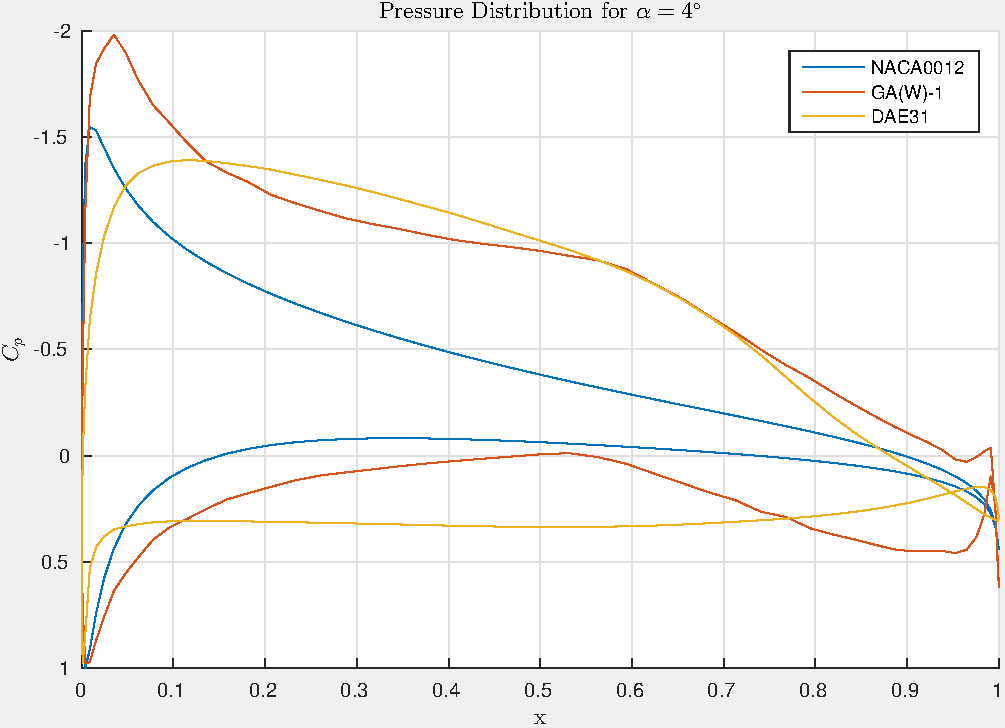
\includegraphics[width = 0.95\textwidth]{./figures/q4pressure.pdf}
    \caption{Pressure Distribution at $\alpha = 4^\circ$}
    \label{fig:q4c}
\end{figure}


\subsection*{(d) Skin Friction Coefficient and Transition}
\begin{figure}[!th]
    \centering
    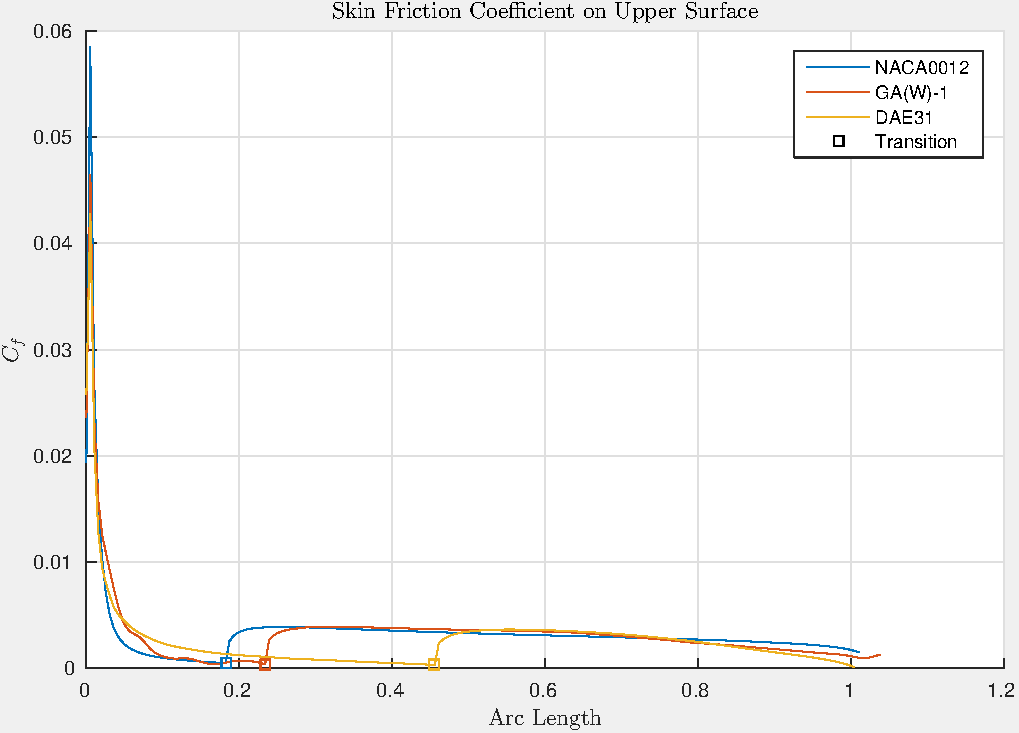
\includegraphics[width = 0.85\textwidth]{./figures/q4uppercf.pdf}
    \caption{Skin Friction Coefficient on Upper Surface at $\alpha = 4^\circ$}
    \label{fig:q4dupper}
\end{figure}

\begin{figure}[!th]
    \centering
    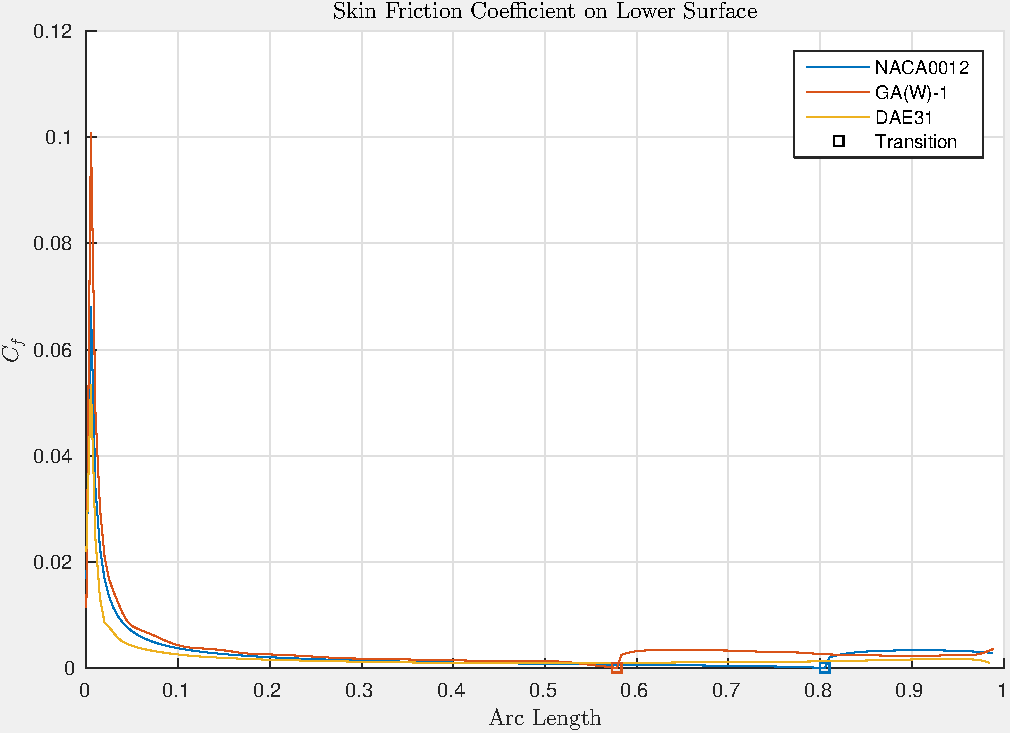
\includegraphics[width = 0.85\textwidth]{./figures/q4lowercf.pdf}
    \caption{Skin Friction Coefficient on Lower Surface at $\alpha = 4^\circ$}
    \label{fig:q4dlower}
\end{figure}

Figure \ref{fig:q4dupper} and \ref{fig:q4dlower} show the skin friction drag coefficient along the arclength and where the laminar-to-turbulent transition occurs for an AoA $\alpha = 4^\circ$.
Since skin friction drag is the only source of drag in this numerical solution, more drag will be generated by turbulent regions.
Therefore, the earlier the transition, the more drag the airfoil will generate.

On the upper surface, the NACA0012 becomes turbulent before both the GA(W)-1 and the DAE31. The DAE31 stays laminar for much longer than the other two airfoils. The DAE31 stays fully laminar on its lower surface, while the GA(W)-1 transitions before the NACA0012 on the lower surface.

At an AoA $\alpha = 4^\circ$ the DAE31 has the lowest drag coefficient, followed by the NACA0012, followed by the GA(W)-1.
The DAE31 obviously has less drag since it transitions much later than the other two.
The NACA0012 transitions slightly later than the GA(W)-1 on the upper surface, but much later on its lower surface, resulting in a lower total drag for the NACA0012.


\section*{Question 5}
\subsection*{(a) Effect of Thickness}

Figure \ref{fig:q5apressure} shows the pressure distribution for varying thicknesses of the 4 digit NACA00XX.

As thickness increases, the laminar-to-turbulent transition moves upwind until there is a laminar separation bubble for a thickness of 20\%.
For thicknesses of 24\% and 26\%, there is a turbulent separation near the TE.
The change in the transition location can be explained by the longer arclength traveled by the fluid when the airfoil is thicker.

Figure \ref{fig:q5adrag} shows that an increasing AoA increases drag. This is expected since the transition happens earlier, leading to a larger turbulent region which finally leads to a higher skin friction drag coefficient.

\begin{figure}[!h]
    \centering
    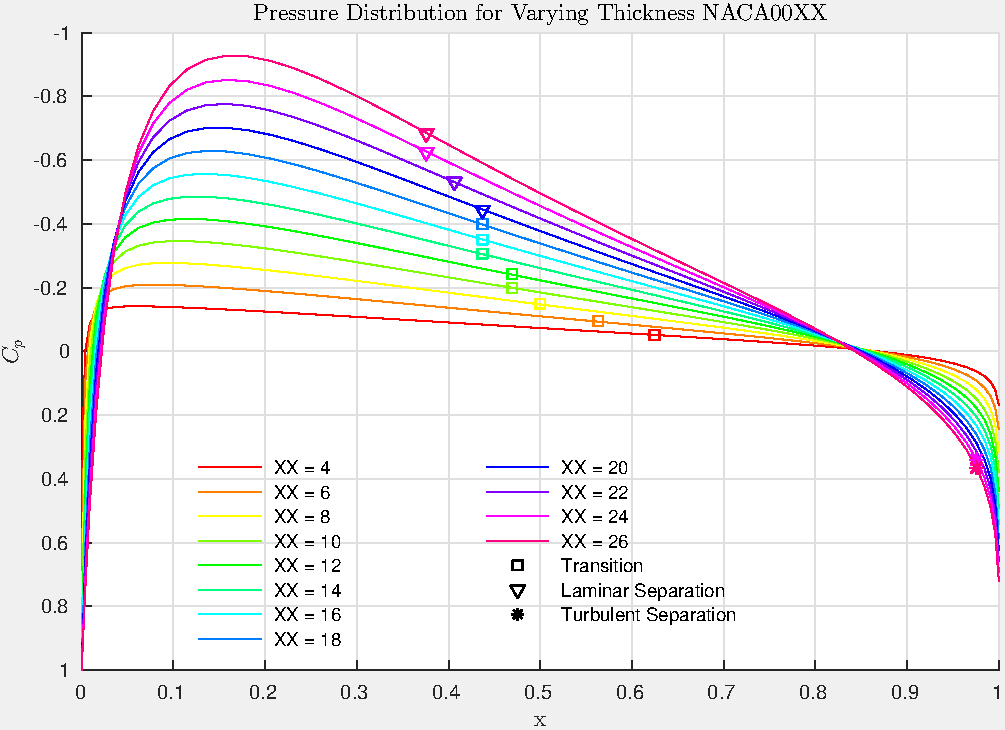
\includegraphics[width = 0.85\textwidth]{./figures/q5apressure.pdf}
    \caption{Pressure Distribution for Variable Thickness}
    \label{fig:q5apressure}
\end{figure}

\begin{figure}[!h]
    \centering
    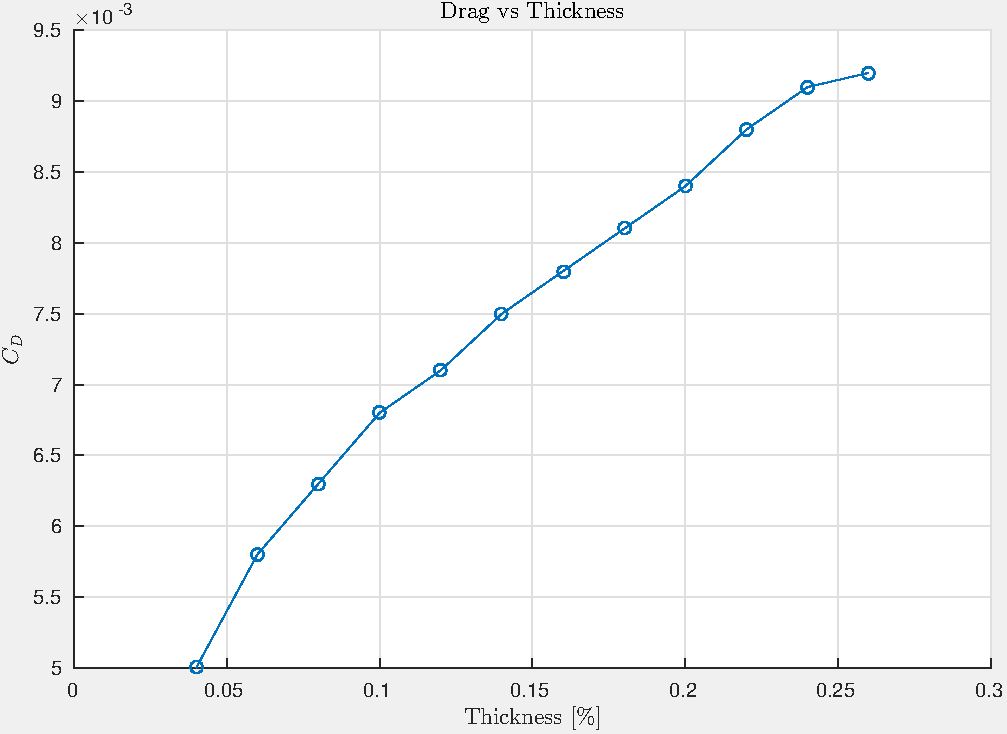
\includegraphics[width = 0.85\textwidth]{./figures/q5dthick.pdf}
    \caption{Effect of Thickness on Drag}
    \label{fig:q5adrag}
\end{figure}

\subsection*{(b) Effect of Maximum Camber}

Figure \ref{fig:q5apressure} shows the pressure distribution for varying maximum camber of the 4 digit NACAX412.

As the camber increases, the top surface transition location does not change by much until laminar separation occurs at a maximum camber of 0.06\%.
The lower surface transition is much more affected by the maximum camber and a separation bubble also occurs for a camber of 0.06\%.

Since the transition occurs earlier as the maximum camber increases, the drag coefficient is expected to increase with camber. This is confirmed by Figure \ref{fig:q5bdrag}.

\begin{figure}[!h]
    \centering
    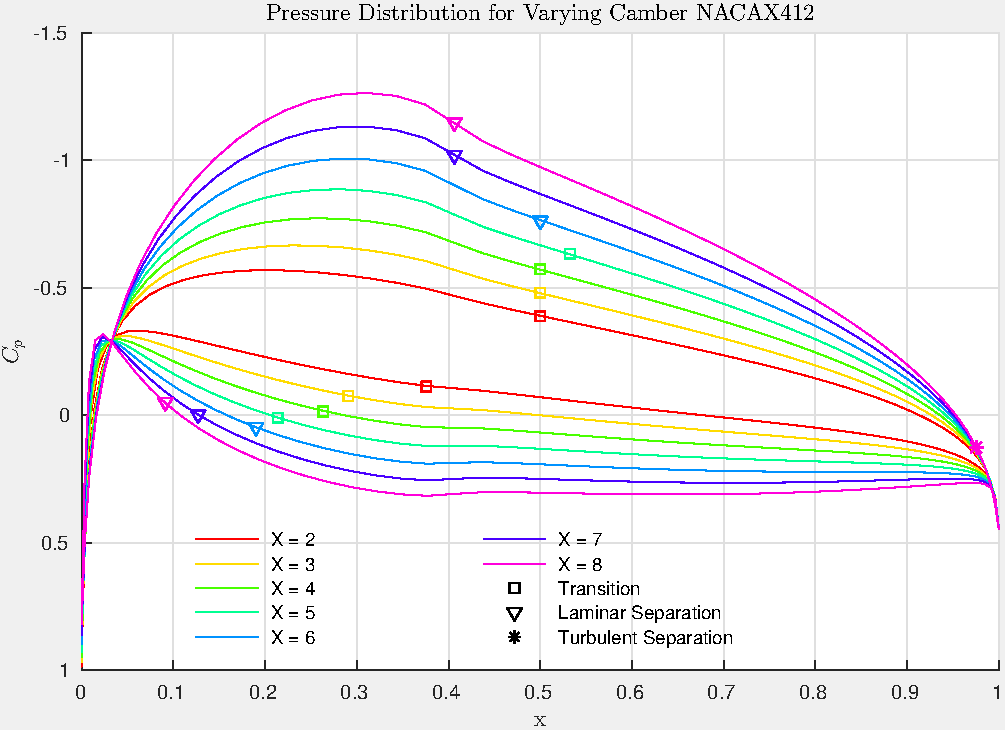
\includegraphics[width = 0.85\textwidth]{./figures/q5bpressure.pdf}
    \caption{Pressure Distribution for Variable Maximum Camber}
    \label{fig:q5bpressure}
\end{figure}

\begin{figure}[!h]
    \centering
    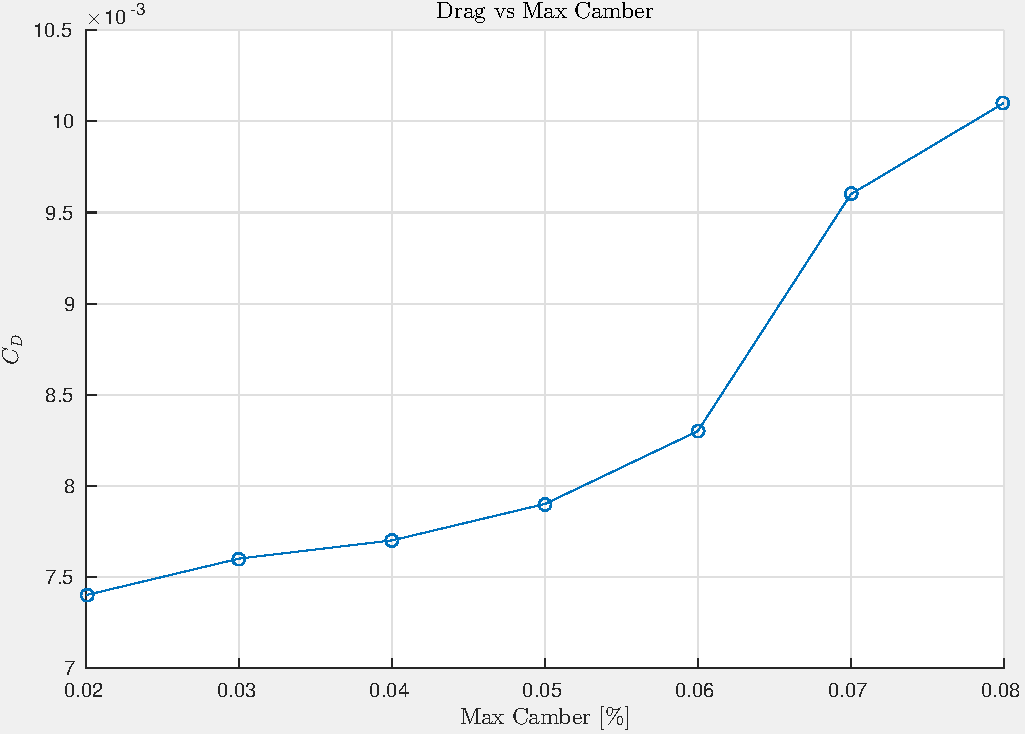
\includegraphics[width = 0.85\textwidth]{./figures/q5dmaxcam.pdf}
    \caption{Effect of Maximum Camber on Drag}
    \label{fig:q5bdrag}
\end{figure}
\clearpage
\subsection*{(c) Effect of Camber Location}
Figure \ref{fig:q5apressure} shows the pressure distribution for varying maximum camber location of the 4 digit NACA4X12.

The lower surface transition moves aft as the maximum camber location goes to the TE. Leading to a lower skin friction drag. However the upper surface transition moves downwind and then upwind, leading to an optimal camber location for minimum drag.

It is interesting to note that when the camber occurs too early, laminar separation occurs instead of transition.
\begin{figure}[!h]
    \centering
    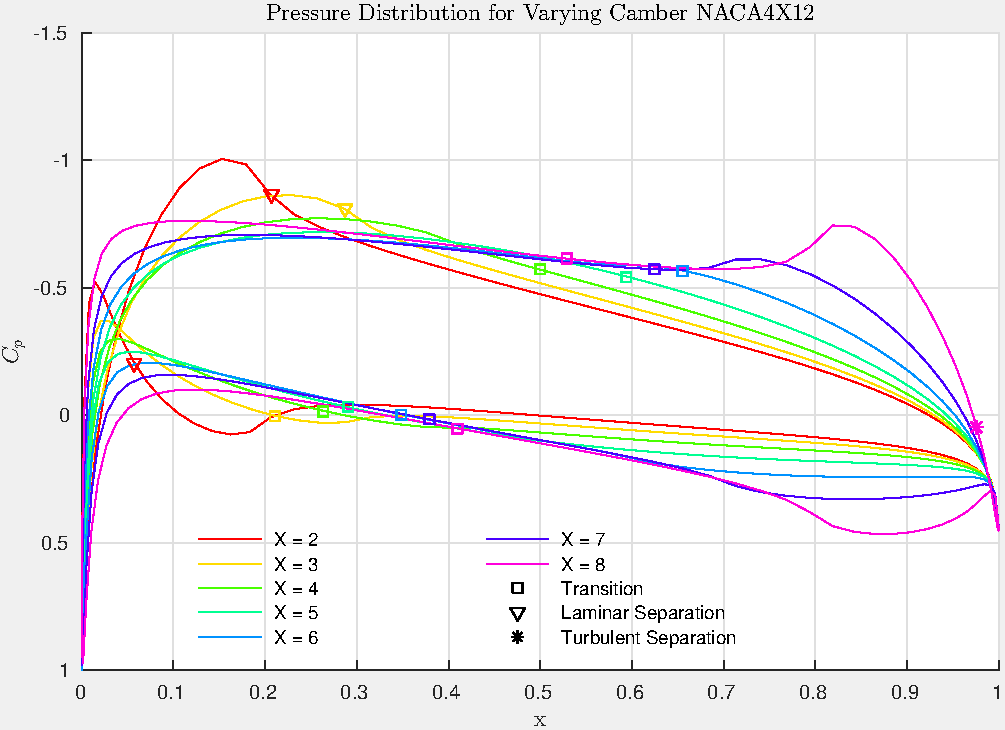
\includegraphics[width = 0.85\textwidth]{./figures/q5cpressure.pdf}
    \caption{Pressure Distribution for Variable Camber Location}
    \label{fig:q5cpressure}
\end{figure}

\begin{figure}[!h]
    \centering
    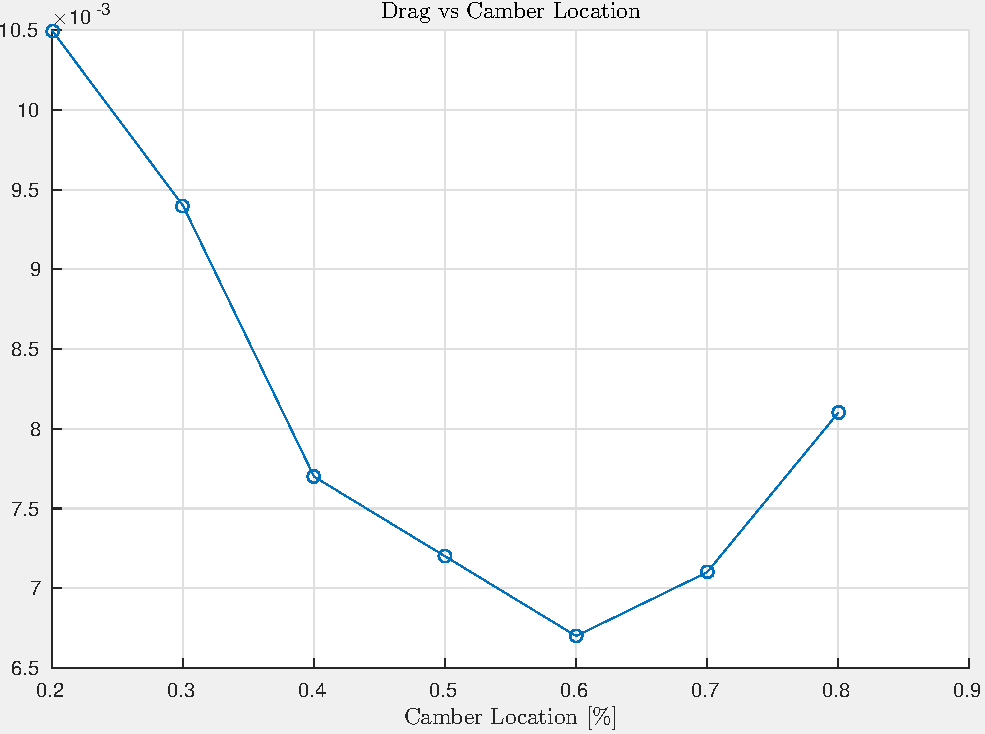
\includegraphics[width = 0.85\textwidth]{./figures/q5dcamloc.pdf}
    \caption{Effect of Camber Location on Drag}
    \label{fig:q5cdrag}
\end{figure}

\end{document}
